\documentclass[11pt]{book}

\usepackage[width=7.0in, height=9.0in, top=1.0in, papersize={8.5in,11in}]{geometry}
\usepackage[pdftex]{graphicx}
%\usepackage{datetime}
\usepackage{anyfontsize}
\usepackage{t1enc}
\usepackage{verbatim}
\usepackage{algorithm}
\usepackage{algorithmic}
\usepackage{framed}
\usepackage{pdfpages}
\usepackage[export]{adjustbox}
\usepackage{listings}
\lstset{language=C}

\lstset{language=python,frame=ltrb,framesep=5pt,basicstyle=\normalsize,
 keywordstyle=\ttfamily\color{DarkRed},
%morecomment=[n][\textbf]{In\ [}{]\:},
%morecomment=[n][\textbf]{Out\ [}{]\:},
morecomment=[s][\color{blue}]{In\ [}{]\:},
morecomment=[s][\color{red}]{Out[}{]\:},
identifierstyle=\ttfamily\color{DarkBlue}\bfseries,
commentstyle=\color{DarkGreen},
stringstyle=\ttfamily,
showstringspaces=false,tabsize = 3}


\lstdefinelanguage{shell} {
commentstyle = \color{black},
keywordstyle = \color{black},
stringstyle = \color{black},
identifierstyle = \color{black},
morecomment=[s][\color{blue}]{In\ [}{]\:},
morecomment=[s][\color{red}]{Out[}{]\:},
 }

\pagestyle{empty}

%\usepackage{helvet}
\renewcommand{\familydefault}{\sfdefault}

\begin{document}

\section*{Team Overview}
\hrulefill
\subsection*{Members}
Mackenzie Smith, Alex Nienhueser

\subsection*{Project Title}
Dahl Virtual Museum Tour

\subsection*{Company}
Dahl Arts Center


\section*{Sprint Report}
\hrulefill
\subsection*{Work Accomplished}
\begin{itemize}
\item Implemented pop-up text descriptions
\item Applied new textures to floor and walls
\item Decided to add another feature for on-rails tour (will be discussed later)


\end{itemize}
\subsection*{Work Left}
\begin{itemize}
\item User documentation
\item Obtain missing art pieces from Dahl
\item Fix issue of video and sound synchronization
\item Research into alternate environments
\end{itemize}

\section*{Sprint Overview}
Text descriptions were the main feature to be implemented into the gallery for this sprint.  While each description box does not have the corresponding description, the methods are there to ensure easy application for when the Dahl has the text finalized.  Another feature which originated from an idea Alex had, was to have a sort of menu system in the on-rails tour to facilitate quick transitions to any desired painting, rather than having to wade through all of the previous ones. Dr. Adkins does not know about this yet as it was within the last week of the sprint that it was started. 

\section*{Text Descriptions}
What has been called "text descriptions" are a combination of two elements.  One being an excerpt written by someone at the Dahl Arts Center designed to give insight into the corresponding painting.  The second element is the object in the Unreal Engine designed to display the previously described description.  This sprint was focused on building the second element, the Unreal Engine object.  The main feature associated with these descriptions is when the user looks at the object, it will play an animation of the object coming out of the wall to a readable distance from the user.  

This was done by making a rectangular object in the engine, then applying a blueprint to each object to have it come out from the wall into a readable distance from the user.  There will be screenshots of the object before animation and after to illustrate the difference.

\section*{Menu System}
This section describes the feature thought up by Alex, which will make navigating through the on-rails tour much more user-friendly.  The way it will work is: the user will press a button to open the menu and the menu will slowly fade into the user's view frame.  The menu itself will compose of a rectangular object which will scroll left to right or right to left, displaying the list of available paintings on top of that rectangular object.  An arrow will point to the selected painting to avoid any ambiguity as to which painting the user wants to jump to.  This feature will be finalized during the last two sprints.

\section*{Client Interactions}
The only meeting with Dr. Adkins was at the beginning of the sprint to go over what was going to be done during this sprint.  There should have been more meetings with him to discuss the menu system, the fault is with the senior design team for not communicating well enough.

\section*{Code Samples}

	\begin{figure}
		\caption{This code section's purpose is to get the user's viewing vector}
		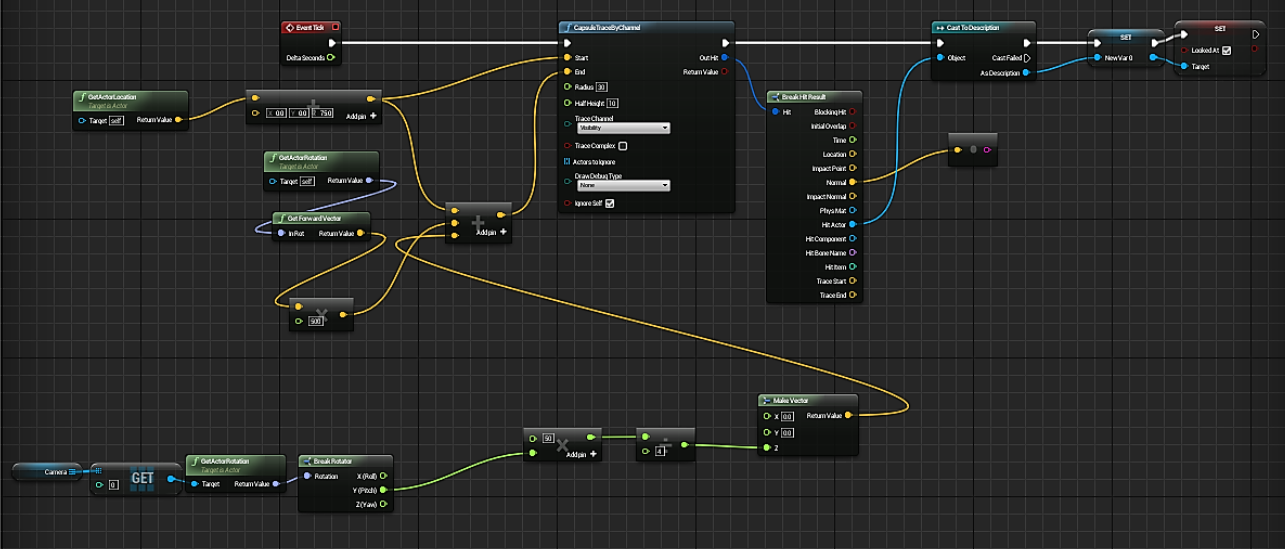
\includegraphics[scale=0.5]{TextDescription1.png}
		\centering
	\end{figure}
	\begin{figure}
		\caption{Animation blueprint for the text description box}
		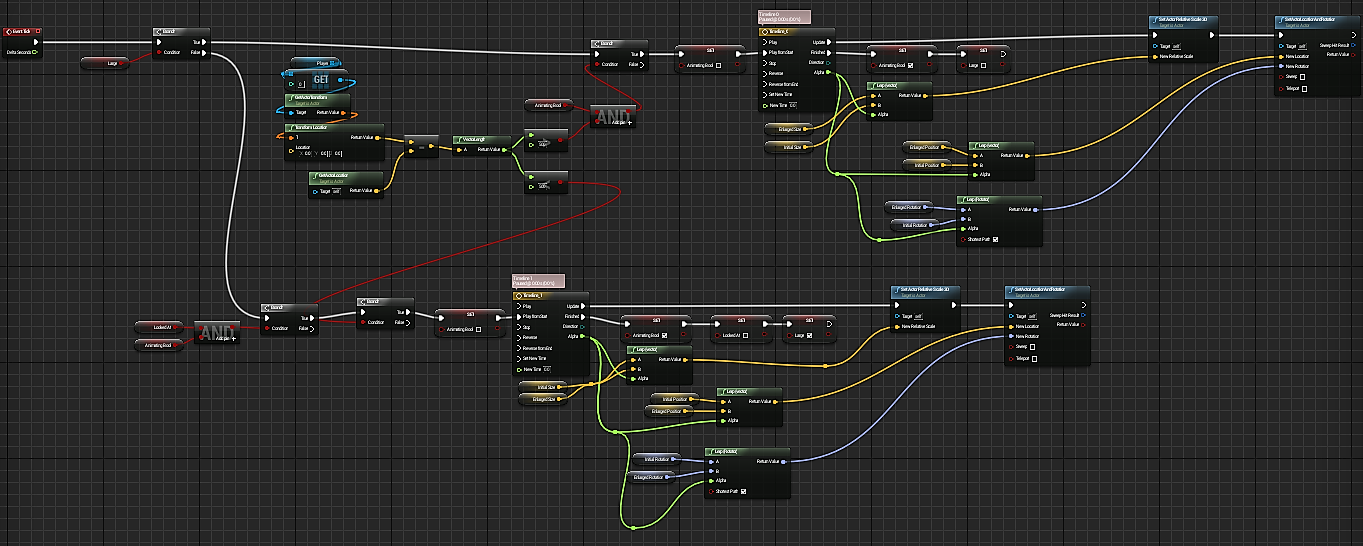
\includegraphics[scale=0.5]{TextDescription2.png}
		\centering
	\end{figure}
	\begin{figure}
		\caption{First half of blueprint that minimizes the description box}
		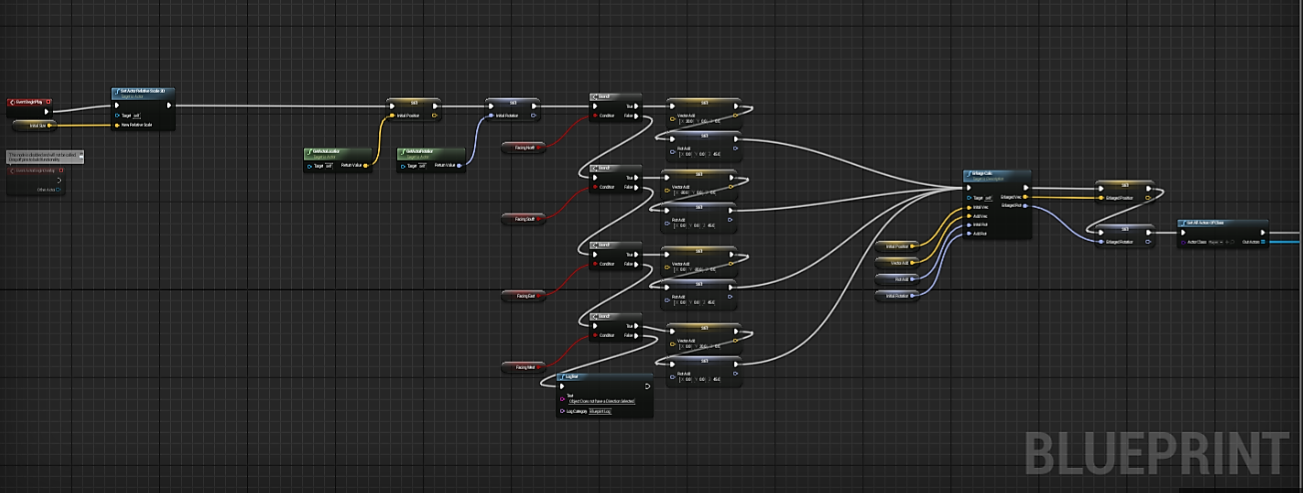
\includegraphics[scale=0.5]{TextDescription3.png}
		\centering
	\end{figure}
	\begin{figure}
		\caption{Second half of minimizing blueprint}
		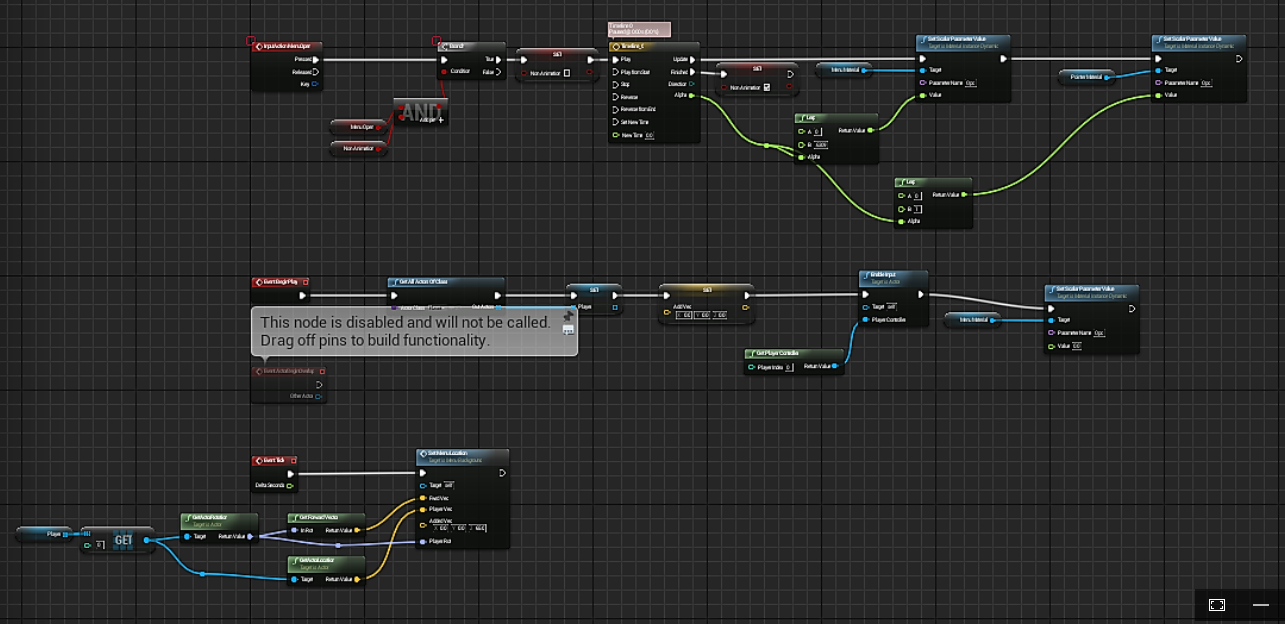
\includegraphics[scale=0.5]{TextDescription4.png}
		\centering
	\end{figure}
	
	\begin{figure}
		\caption{Displays the menu in the center of the user's vision}
		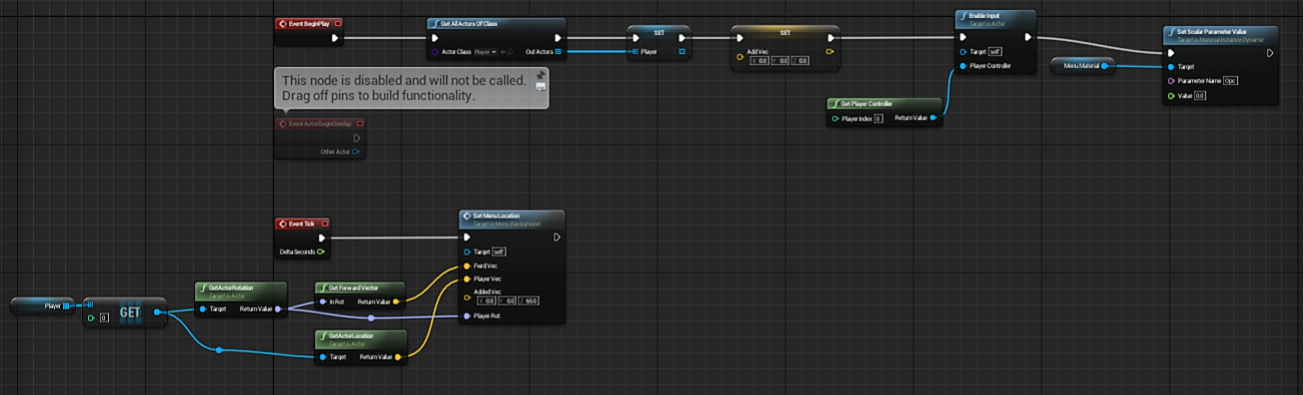
\includegraphics[scale=0.5]{Menu1.png}
		\centering
	\end{figure}
	\begin{figure}
		\caption{Allows navigation in the menu}
		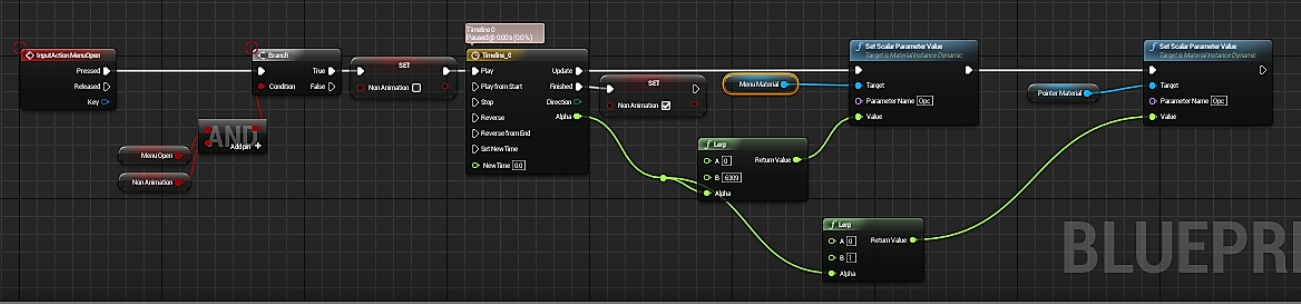
\includegraphics[scale=0.5]{Menu2.png}
		\centering
	\end{figure}

\section*{Screenshots}
	\begin{figure}
		\caption{Description box is initially flush with the wall}
		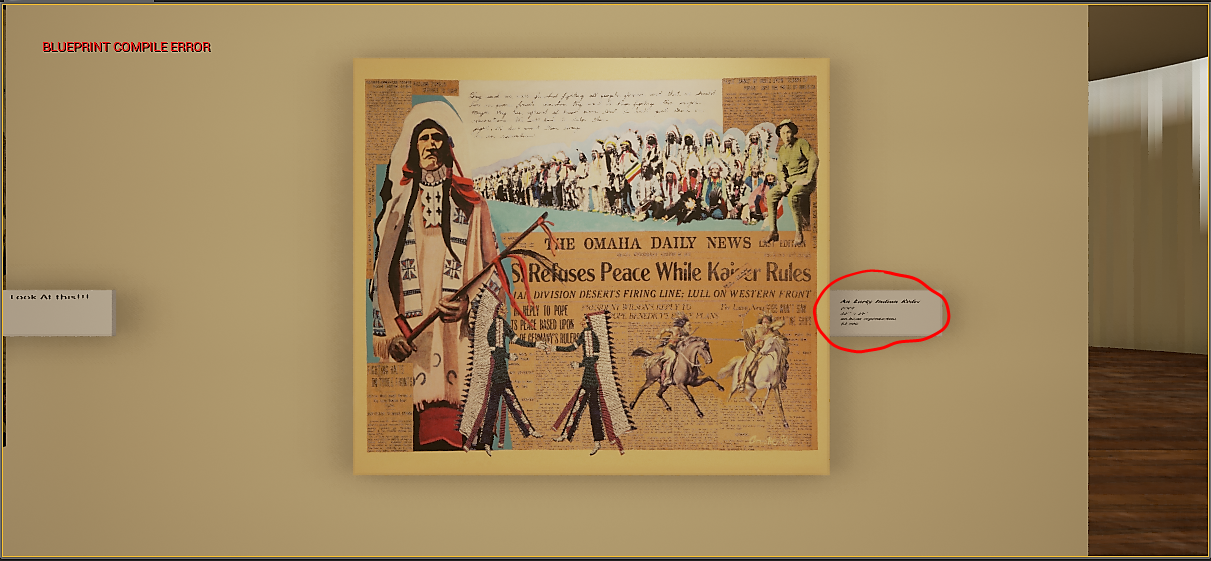
\includegraphics[scale=0.5]{Screenshots/Animation1.png}
		\centering
	\end{figure}
	\begin{figure}
		\caption{The description box then starts to come out from the wall}
		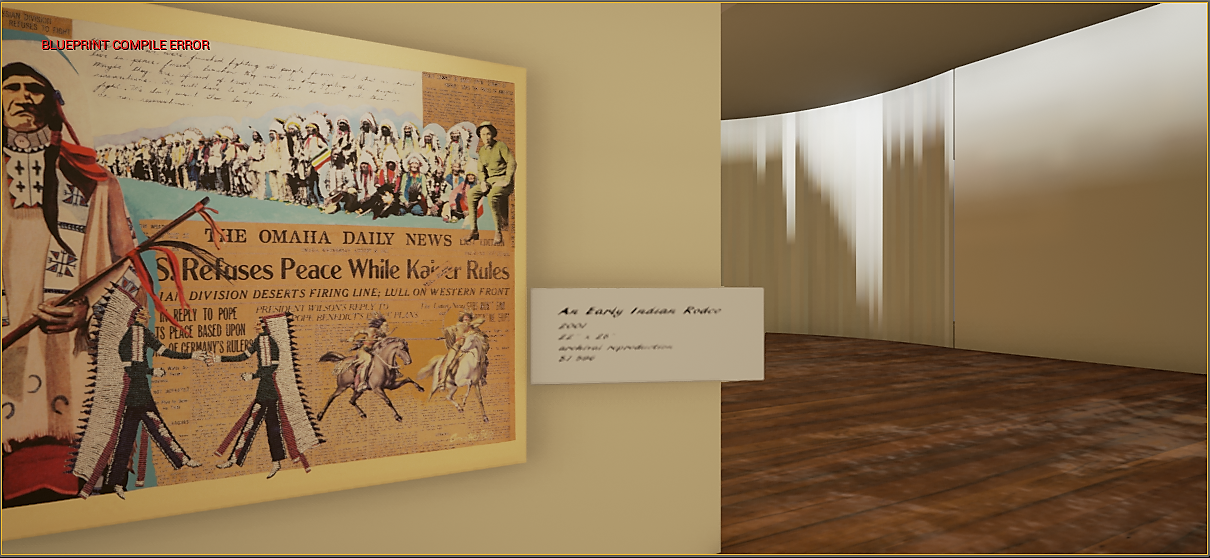
\includegraphics[scale=0.5]{Screenshots/Animation2.png}
		\centering
	\end{figure}
	\begin{figure}
		\caption{After the box ends its forward animation}
		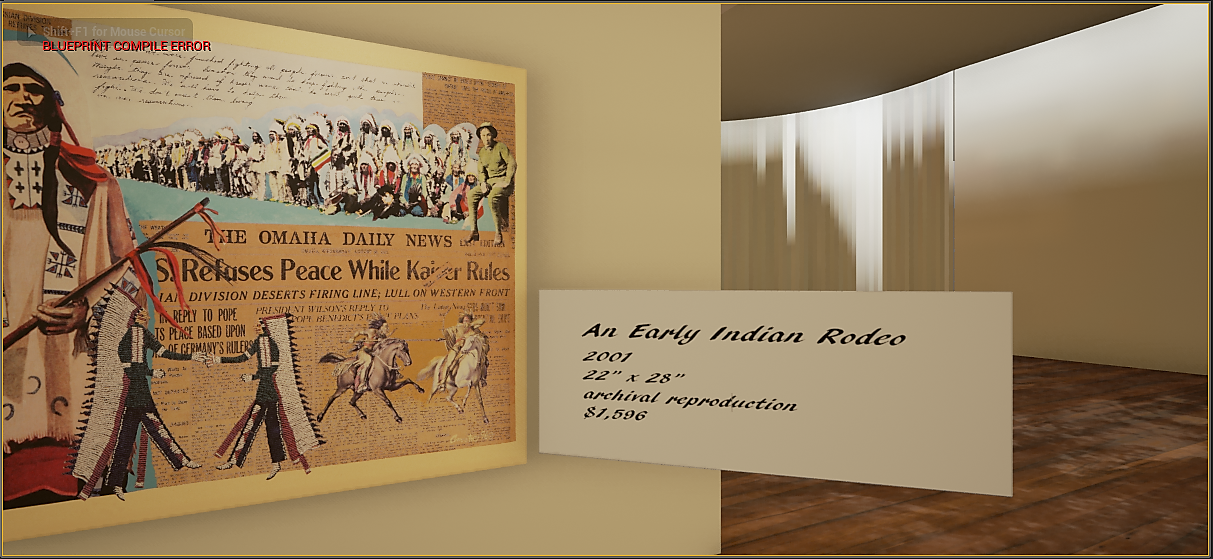
\includegraphics[scale=0.5]{Screenshots/Animation3.png}
		\centering
	\end{figure}
	\begin{figure}
		\caption{When the user walks a certain distance away, the box will start to shrink back}
		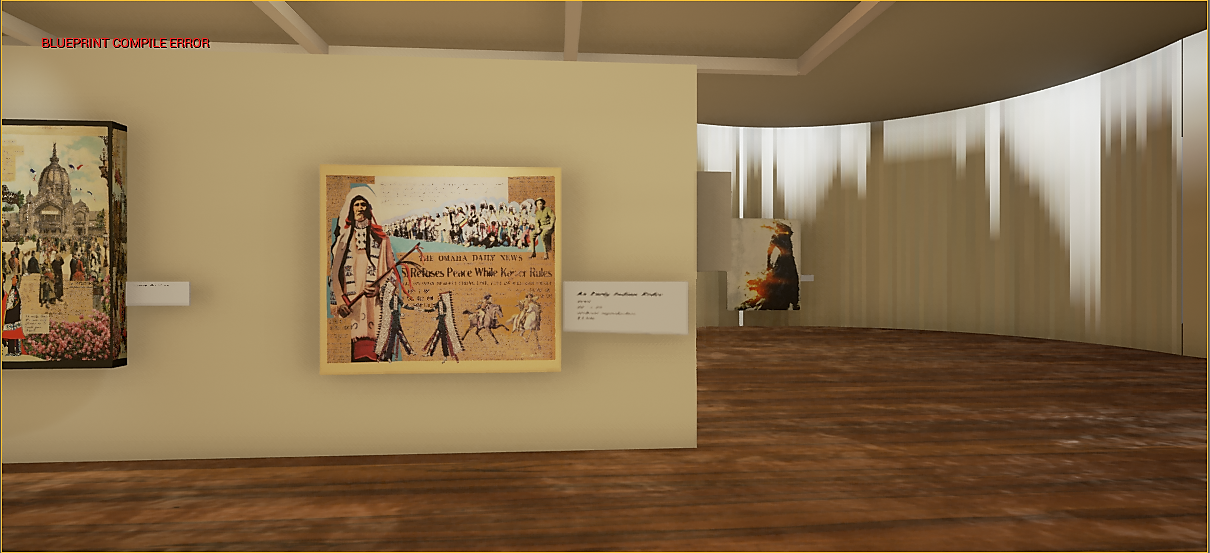
\includegraphics[scale=0.5]{Screenshots/Animation4.png}
		\centering
	\end{figure}
	\begin{figure}
		\caption{Final resting place of the description box}
		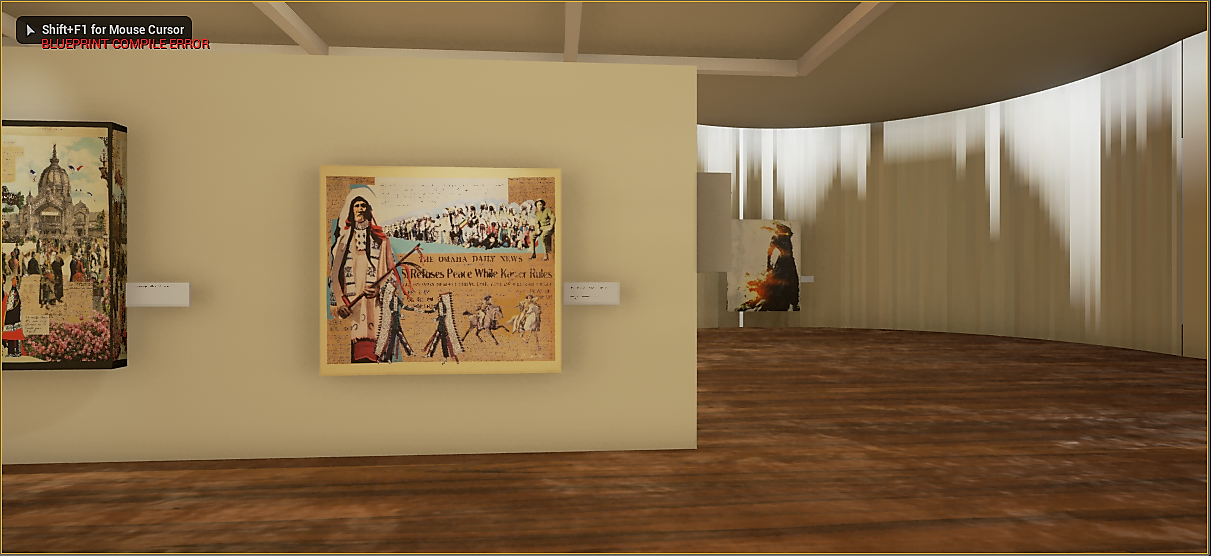
\includegraphics[scale=0.5]{Screenshots/Animation5.png}
		\centering
	\end{figure}


	\begin{figure}
		\caption{The small triangle will indicate which painting is currently selected}
		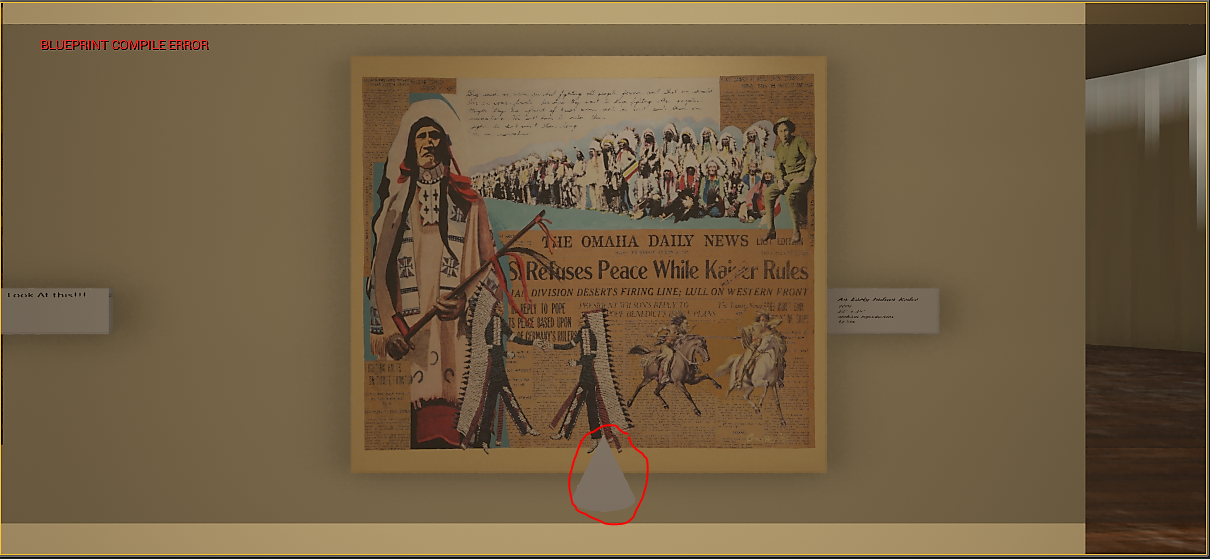
\includegraphics[scale=0.5]{Screenshots/Menu.png}
		\centering
	\end{figure}

\section*{Issues}
The only issue that happened during this sprint was the missing descriptions from the Dahl, which was communicated to Dr. Adkins after the end of the sprint.  This will be fixed in the last two sprints.

\end{document}
